\begin{titlepage}

\center{\fontsize{4cm}{5cm}\selectfont VOTCA}
\center{\fontsize{1.5cm}{3cm}\selectfont USER MANUAL}

\vspace*{3cm}
\center{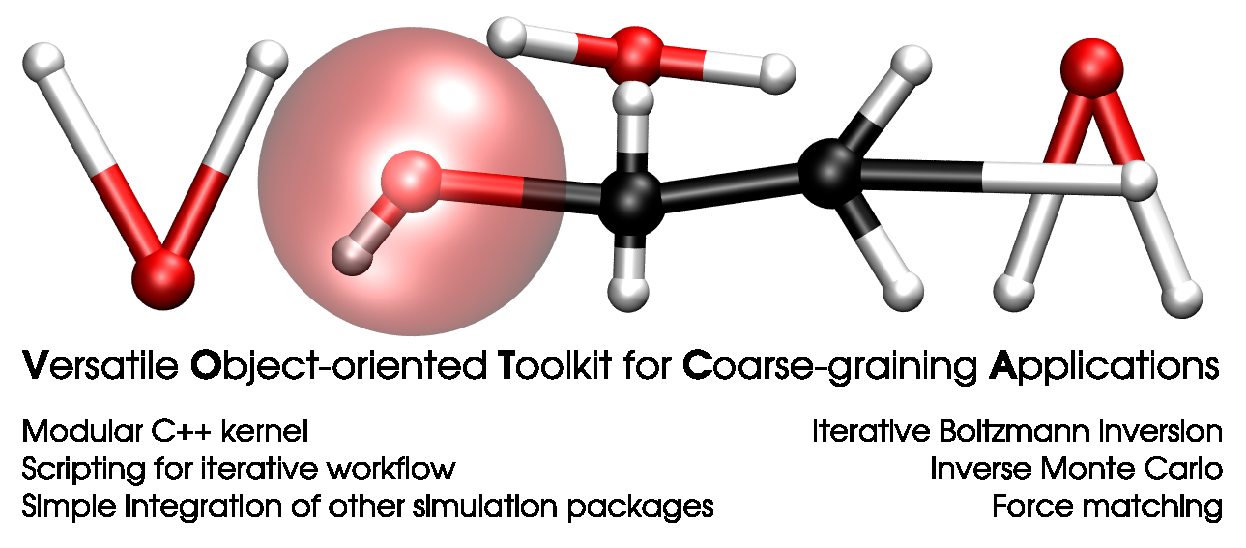
\includegraphics[width=\columnwidth]{fig/logo}}
\vspace*{1cm}
\vfill
\vspace*{1.4cm}
\center{\large{\today}}
\vspace*{-0.3cm}
\center{\footnotesize{Version: \gitid}}
\center{\footnotesize{Programs version: \csgid}}

\vspace*{1cm}
%\center{
\large{\copyright \hspace*{0.1cm} VOTCA development team}
%}
\vspace*{0.5cm}

\htmladdnormallink{\color{black}\large{www.votca.org}}{http://www.votca.org}
\end{titlepage}

\section*{Disclamer}
This manual is not complete. The best way to start using the software is to look at provided tutorials. The reference section is generated automatically from the source code, so please make sure that your software and manual versions match.  

\section*{Citations}
Development of this software depends on academic research grants. If you are using the package, please cite the  following papers \\

\vspace{0.1cm}
\noindent
\cite{mashayakrelative} Relative entropy and optimization-driven coarse-graining methods in VOTCA, \\
S.Y. Mashayak, Mara Jochum, Konstantin Koschke, N.R. Aluru, Victor R\"uhle, and Christoph Junghans,\\
\htmladdnormallink{  {\itshape Plos One} (2015)}
{http://dx.doi.org/10.1371/journal.pone.0131754}

\vspace{0.1cm}
\noindent
\cite{ruhle2011hybrid} Hybrid approaches to coarse-graining using the VOTCA package: liquid hexane, \\
Victor R\"uhle and Christoph Junghans, \\
\htmladdnormallink{  {\itshape Macromol. Theory Simul.} 20, 472 (2011)}
{http://dx.doi.org/10.1002/mats.201100011}

\vspace{0.1cm}
\noindent
\cite{Ruehle:2009.a} Versatile Object-oriented Toolkit for Coarse-graining Applications \\
Victor R\"uhle, Christoph Junghans, Alexander Lukyanov, Kurt Kremer, and Denis Andrienko \\
\htmladdnormallink{  {\itshape J. Chem. Theor. Comp.} 5, 3211, 2009}
{http://dx.doi.org/10.1021/ct900369w}

\section*{Development}
The core development is currently taking place at the Los Alamos National Laboratory and Max Planck Institute for Polymer Research, Mainz, Germany.

\section*{Copyright}
\votca is free software. The entire package is available under the Apache License. For details, check
the LICENSE file in the source code. The \votca source code is available on our homepage, \htmladdnormallink{\color{black}www.votca.org}{http://www.votca.org}.

\vfill
